\subsection{Những hàm số sơ cấp}

\ % Lùi đầu dòng

Trong phần này, các hàm số quen thuộc sẽ được nhắc lại. Đây là những hàm hay thấy nhất trong quá trình học phần lớn các môn khoa học tự nhiên.

\subsubsection{Đa thức}
Đầu tiên, chúng ta có hàm \emph{đa thức}, thông thường được biểu diễn dưới dạng $$f(x)=P_n(x)=\sum_{i = 0}^n a_i x^i = a_nx^n + a_{n-1}x^{n-1} + \cdots + a_1x + a_0$$ với $n$ là một số nguyên không âm, $a_i$ là các số thực, gọi là các \emph{hệ số}, với mọi $i$ nguyên nằm trong đoạn $[0, n]$ và $a_n \neq 0$. Khi này, $n$ được gọi là \emph{bậc} của đa thức. Ví dụ:
\begin{itemize}
   \item $f(x) = 2x^2 + 3x + 1$ là một đa thức bậc $2$ với các hệ số $a_2 = 2$, $a_1 = 3$, $a_0 = 1$;
   \item $g(y) = y^3 - 4y$ là một đa thức bậc $3$ với các hệ số $b_3 = 1$, $b_2 = 0$, $b_1 = -4$, $b_0 = 0$;
   \item $h(z) = 5$ là một đa thức bậc $0$ với hệ số $c_0 = 5$;
\end{itemize}
Tính toán một số giá trị mẫu:
\begin{itemize}
   \item $p(1) = 7 \cdot 1^4 - 2 \cdot 1^2 + 9 = 14$ với $q(t)= 7t^4 - 2t^2 + 9$ là một đa thức bậc $4$ với các hệ số $d_4 = 7$, $d_3 = 0$, $d_2 = -2$, $d_1 = 0$, $d_0 = 9$;
   \item $q(2) = -3 \cdot 2 + 8 = 2$ với $q(r) = -3r + 8$ là một đa thức bậc $1$ với các hệ số $e_1 = -3$, $e_0 = 8$.
\end{itemize}
Khi đa thức có bậc bằng $0$, hay $f(x) = P_0(x) = a_0$, thì được gọi là \emph{đa thức hằng} hay \emph{hàm hằng}. Một trường hợp đặc biệt là khi $f(x) = 0$ \footnote{Sẽ có nhiều tài liệu viết \dblquote{$f(x) \equiv 0$} thay vì \dblquote{$f(x) = 0$} để phân biệt giữa khẳng định hai hàm là như nhau so với một phương trình. Tác giả không muốn bạn đọc phải bận tâm với nhiều kí hiệu lạ, cho nên tác giả sẽ cố gắng dùng những kí hiệu cũ. Bạn đọc có thể tự suy luận ý nghĩa thông qua ngữ cảnh.}. Nếu hàm này là đa thức, theo định nghĩa, hàm này có bậc là $0$ và hệ số $a_0 = 0$. Tuy nhiên, cũng theo định nghĩa thì hệ số đầu phải khác $0$. Vì vậy, hàm không có bậc và không được gọi là đa thức. Nhưng, do hàm nhận giá trị cố định với mọi $x$ nên vẫn được gọi là hàm hằng \footnote{Đa số những nhà toán học không coi $f(x) = 0$ là đa thức bậc $0$ do nhiều tính chất của đa thức bị phá vỡ khi gặp trường hợp này. Do đó, $f(x) = 0$ chỉ được coi là \dblquote{hàm hằng} chứ không phải \dblquote{\textit{đa thức} hằng}. Trong tài liệu này, trở về sau sẽ chỉ có thuật ngữ \dblquote{hàm hằng} được sử dụng.}.

\exercise Phác thảo đồ thị của những hàm sau:
\begin{multicols}{2}
\begin{enumerate}
   \item $f(x) = x + 2$; 
   \item $f(x) = x^2 + 2x + 3$;
   \item $f(x) = x^3 - 9x^2 + 24x - 16$;
   \item $f(x) = 2$.
\end{enumerate}
\end{multicols}

\solution

Khả năng rất cao là bạn đọc có kết nối với mạng; vì vậy, bạn đọc có thể dùng những phần mềm vẽ đồ thị để nhanh chóng có hình vẽ. Tuy nhiên, nếu không có thiết bị điện tử thì bạn đọc vẫn có thể vẽ đồ thị bằng giấy và bút bằng cách lấy nhiều điểm ví dụ cho $x$ và tính toán giá trị $f(x)$ và sau đó nối chúng lại với nhau.

Bạn đọc có thể để ý rằng là không phải lúc nào cũng đặt gốc tọa độ ở vị trí chính giữa. Trong nhiều trường hợp việc đặt chính giữa sẽ làm mất đi đồ thị và làm cho đồ thị lệch ra khỏi khu vực vẽ. Hơn nữa, hai trục sẽ có tỉ lệ khác nhau. Điều quan trọng nhất của những bài vẽ đồ thị trong vật lí không phải là căn ke chính xác vị trí từng điểm, mà là nhận ra được dáng điệu của đồ thị và vị trí tương đối giữa các điểm trên đồ thị đó. Qua đó, chúng ta rút ra được những tính chất toán học cần thiết để phục vụ những yêu cầu cụ thể trong bài toán.

Dưới đây là đồ thị của các hàm đa thức trong bài:

\begin{figure}[H]
   \centering
   \begin{minipage}[t]{0.48\textwidth}
      \centering
      \fbox{
         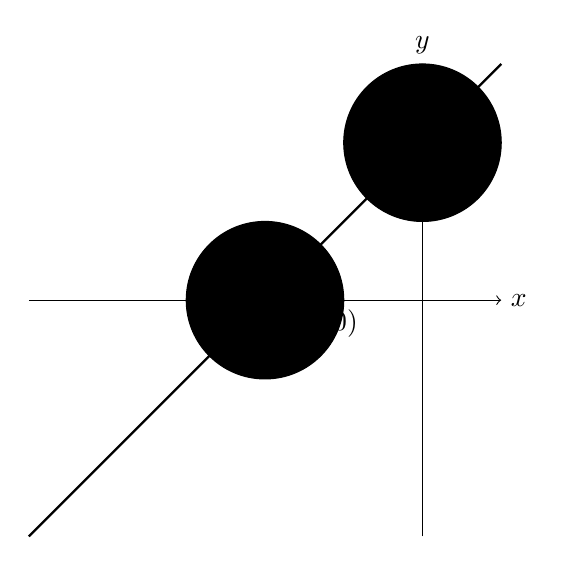
\begin{tikzpicture}
            \draw[->] (-5, 0) -- (1, 0) node[right] {$x$};
            \draw[->] (0, -3) -- (0, 3) node[above] {$y$};
            \draw[thick] plot[domain=-5:1] (\x, {\x + 2});
            \filldraw (0, 2) circle (\pointSize) node[below right] {$\left(0; 2\right)$};
            \filldraw (-2, 0) circle (\pointSize) node[below right] {$\left(-2; 0\right)$};
         \end{tikzpicture}
      }
      \caption{Đồ thị của hàm $f(x) = x + 2$}
      \label{fig:ham_so:ham_so_cap:x_2}
   \end{minipage}
   \hfill
   \begin{minipage}[t]{0.48\textwidth}
      \centering
      \fbox{
         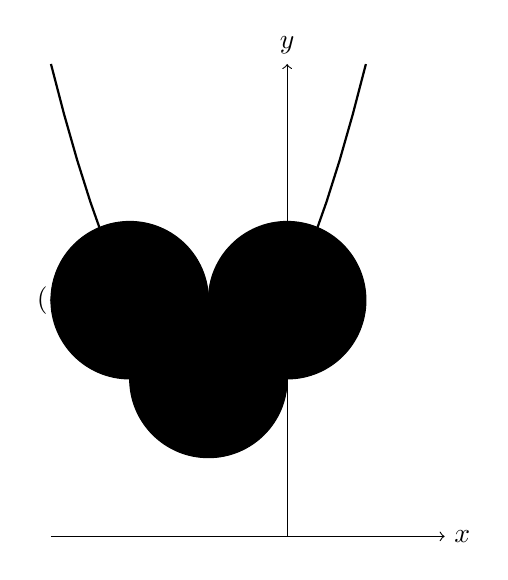
\begin{tikzpicture}
            \draw[->] (-3, 0) -- (2, 0) node[right] {$x$};
            \draw[->] (0, 0) -- (0, 6) node[above] {$y$};
            \draw[thick] plot[domain=-3:1] (\x, {(\x + 1)^2 + 2});
            \filldraw (-1, 2) circle (\pointSize) node[below] {$\left(-1; 2\right)$};
            \filldraw (0, 3) circle (\pointSize) node[below right] {$\left(0; 3\right)$};
            \filldraw (-2, 3) circle (\pointSize) node[left] {$\left(-2; 3\right)$};
         \end{tikzpicture}
      }
      \caption{Đồ thị của hàm $f(x) = x^2 + 2x + 3$}
      \label{fig:ham_so:ham_so_cap:x2_2x_3}
   \end{minipage}
\end{figure}
\begin{figure}[H]
   \centering
   \begin{minipage}[t]{0.48\textwidth}
      \centering
      \fbox{
         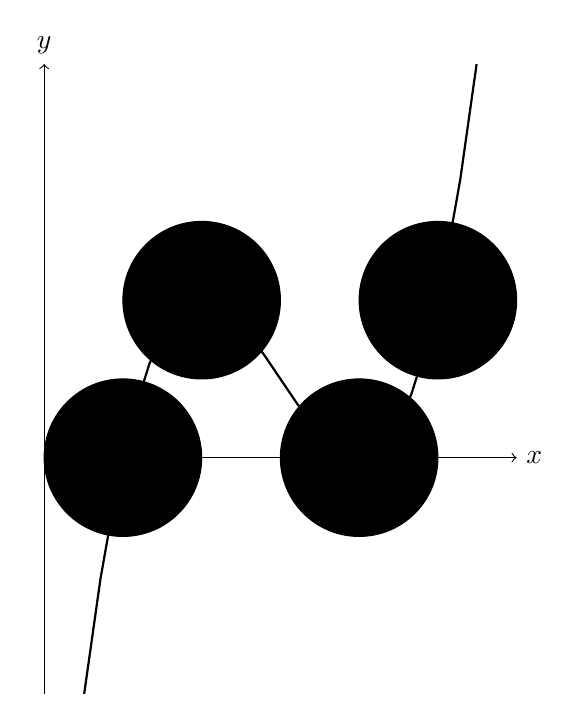
\begin{tikzpicture}
            \draw[->] (0, 0) -- (6, 0) node[right] {$x$};
            \draw[->] (0, -3) -- (0, 5) node[above] {$y$};
            \draw[thick] plot[domain=0.508:5.492] (\x, {((\x)^3 - 9*(\x)^2 + 24*(\x) - 16) / 2});
            \filldraw (2, 2) circle (\pointSize) node[above] {$\left(2; 4\right)$};
            \filldraw (4, 0) circle (\pointSize) node[below] {$\left(4; 0\right)$};
            \filldraw (1, 0) circle (\pointSize) node[below right] {$\left(1; 0\right)$};
            \filldraw (5, 2) circle (\pointSize) node[right] {$\left(5; 4\right)$};
         \end{tikzpicture}
      }
      \caption{Đồ thị của hàm $f(x) = x^3 - 9x^2 + 24x - 16$}
      \label{fig:ham_so:ham_so_cap:x3_t9x2_24x_t16}
   \end{minipage}
   \hfill
   \begin{minipage}[t]{0.48\textwidth}
      \centering
      \fbox{
         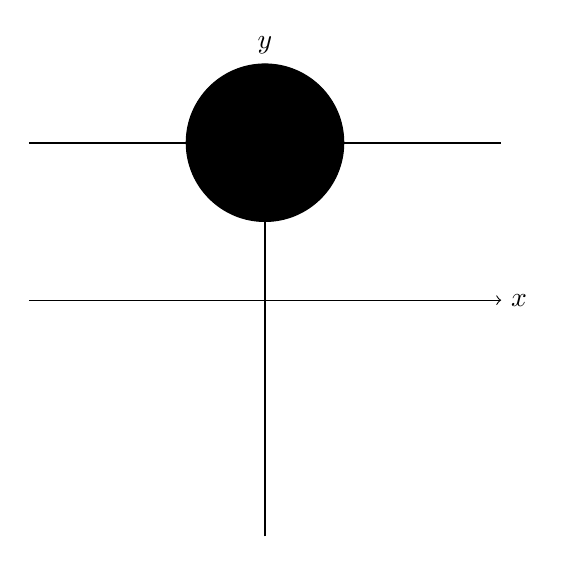
\begin{tikzpicture}
            \draw[->] (-3, 0) -- (3, 0) node[right] {$x$};
            \draw[->] (0, -3) -- (0, 3) node[above] {$y$};
            \draw[thick] plot[domain=-3:3] (\x, {2});
            \filldraw (0, 2) circle (\pointSize) node[above left] {$\left(0; 2\right)$};
         \end{tikzpicture}
      }
      \caption{Đồ thị của hàm $f(x) = 2$}
      \label{fig:ham_so:ham_so_cap:2}
   \end{minipage}
\end{figure}

\exercise Giải những phương trình sau. Các phương trình đều có ẩn là $x \in \mathbb{R}$.
\begin{multicols}{2}
   \begin{enumerate}
      \item $3x - 7 = 0$;
      \item $x - 9 = 5x + 3$;
      \item $\frac{1}{v}\cdot x - \frac{1}{v} \cdot x_0 = t$, với $v$, $x_0$, $t$ là những tham số thực;
      \item $6x^2 - 5x - 21 = 0$;
      \item $5x^2 - 50x + 125 = 0$;
      \item $x^2 + 2x + 4 = 0$;
      \item $x^2 + 2x + 4 = 8$;
      \item $5x^2 - 20x + 20 = x^2 - 4$;
      \item $\frac{1}{2}kx^2 + \frac{1}{2}mv^2 = \frac{1}{2}kx_0^2$, với $k$, $m$, $v$, $x_0$ là những tham số thực;
      \item $x^3 - \frac{11}{6}\cdot x^2 + x - \frac{1}{6} = 0$;
      \item $2x^3 - 2x^2 + 2x - 2 = 6 + 6x^2$.
   \end{enumerate}
\end{multicols}

\solution

1. Biến đổi tương đương phương trình để có:
\begin{align*}
   3x - 7 &= 0 \\
   \iff 3x &= 7\\
   \iff x &= \frac{7}{3}.
\end{align*}
Vậy tập nghiệm của phương trình là $\boxed{\displaystyle\left\{\frac{7}{3}\right\}}$.

2. Chuyển số hạng có thừa số $x$ về một phía, và số hạng tự do về phía còn lại để được:
\begin{align*}
   x - 9 &= 5x + 3 \\
   \iff (x - 9) + (9 - 5x) &= (5x + 3) + (9 - 5x) \\ 
   \iff -4x &= 12 \\
   \iff x &= -3.
\end{align*}
Vậy tập nghiệm của phương trình là $\boxed{\displaystyle\left\{-3\right\}}$.

3. Để giải phương trình có chứa tham số, chúng ta cần viết lại ẩn $x$ dưới dạng một biểu thức chỉ chứa tham số và hằng số. Cụ thể,
\begin{align*}
   \frac{1}{v}\cdot x - \frac{1}{v} \cdot x_0 &= t \\
   \iff \frac{x}{v} &= t + \frac{x_0}{v} \\
   \iff x &= vt + x_0.
\end{align*}
Vậy nghiệm của phương trình là $\boxed{\displaystyle\left\{vt + x_0\right\}}$.

4. Nếu như bạn đọc chưa biết, nếu như một đa thức $f(x)$ nhận $x = a$ là nghiệm thì $f(x)$ có thể được viết thành tích của $(x - a)$ nhân một đa thức $g(x)$ với bậc nhỏ hơn $1$ so với $f(x)$. Và nếu $g(x)$ lại có nghiệm $x = b$ thì chúng ta có thể viết $g(x) = (x-b)h(x)$ và qua đó có thể viết lại $f(x) = (x-a)(x-b)h(x)$. Một cách tổng quát nhất, nếu như $f(x)$ là phương trình bậc $n$ có $n$ nghiệm $a_1, a_2, \cdots, a_n$ thì có thể viết lại $$f(x) = A \prod_{i=1}^{n} (x - a_i) = A(x - a_1)(x - a_2)\cdots (x - a_n)$$ với $A$ là hệ số của số hạng có bậc lớn nhất trong đa thức $f(x)$.

Nhẩm nghiệm (bằng cách bấm máy tính) phương trình thì có $x = -\frac{3}{2}$ và $x = \frac{7}{3}$. Chúng ta kì vọng có thể viết lại phương trình dưới dạng $6\left(x - \left(-\frac{3}{2}\right)\right)\left(x - \frac{7}{3}\right) = 0$. Thực vậy, thực hiện phân tích nhân tử để có:
\begin{align*}
   &6x^2 - 5x - 21 = 0 \\
   \iff &6x^2 - 14x + 9x - 21 = 0 \\
   \iff &2x(3x - 7) + 3(3x - 7) = 0 \\
   \iff &(2x + 3)(3x - 7) = 0 \\
   \iff &\left[
      \begin{aligned}
         2x + 3 &= 0 \\
         3x - 7 &= 0
      \end{aligned}
   \right.
   \iff \left[
      \begin{aligned}
         x &= -\frac{3}{2} \\
         x &= \frac{7}{3}
      \end{aligned}
   \right..
\end{align*}
Vậy phương trình có nghiệm là $\boxed{\displaystyle\left\{-\frac{3}{2}; \frac{7}{3}\right\}}$.

5.
\begin{align*}
   5x^2 - 50x + 125 &= 0 \\
   \iff 5\left(x^2 - 10x + 25\right) &= 0 \\
   \iff 5(x - 5)^2 &= 0 \\
   \iff x - 5 &= 0 \\
   \iff x &= 5.
\end{align*}

Vậy tập nghiệm của phương trình có một phần tử duy nhất $\boxed{\displaystyle\left\{5\right\}}$.

6. Với những phương trình liên quan tới đa thức bậc hai không thể nhẩm ngay được nghiệm, chúng ta sẽ sử dụng phương pháp tách bình phương. Với phương trình được cho:
\begin{align}
   x^2 + 2x + 4 &= 0 \nonumber\\ 
   \iff x^2 + 2x + 1 &= -3 \nonumber\\
   \iff (x + 1)^2 &= -3. \label{eq:ham_so_mot_bien:ham_so_cap:gptdt6}
\end{align}
Một số thực nhân với chính nó sẽ ra một số không âm. Cho nên phương trình \ref{eq:ham_so_mot_bien:ham_so_cap:gptdt6} không thể đúng. Vậy phương trình \fbox{vô nghiệm} trên tập số thực.

7. 
\begin{align*}
   &x^2 + 2x + 4 = 8 \\ 
   \iff &x^2 + 2x + 1 = 5 \\
   \iff &(x + 1)^2 = 5 \\
   \iff &\left[
      \begin{aligned}
         x + 1 &= \sqrt{5} \\
         x + 1 &= -\sqrt{5}
      \end{aligned}
   \right. \\
   \iff &\left[
      \begin{aligned}
         x &= \sqrt{5} - 1 \\
         x &= -\sqrt{5} - 1
      \end{aligned}
   \right..
\end{align*}
Vậy tập nghiệm của phương trình là $\boxed{\displaystyle\left\{\sqrt{5} - 1; -\sqrt{5} - 1\right\}}$.

8. Phần này tác giả làm khác so với phần 2. Chuyển đổi toàn bộ phương trình về một vế để đưa về dạng phương trình $f(x) = 0$:
\begin{align*}
   &5x^2 - 20x + 20 = x^2 - 4 \\
   \iff &4x^2 - 20x + 24 = 0 \\
   \iff &4\left(x^2 - 5x + 6\right) = 0 \\
   \iff &4\left(x^2 - 2x - 3x + 6\right) = 0 \\
   \iff &4\left(x(x - 2) - 3(x - 2)\right) = 0 \\
   \iff &4(x - 3)(x - 2) = 0 \\
   \iff &\left[
      \begin{aligned}
         x - 3 &= 0 \\
         x - 2 &= 0
      \end{aligned}
   \right. \iff x \in \left\{3; 2\right\}. 
\end{align*}
Vậy phương trình có tập nghiệm $\boxed{\left\{3; 2\right\}}$.

9. Nhân cả hai vế với $2$ để khử phân số trong phương trình:
\begin{align}
   &\frac{1}{2}kx^2 + \frac{1}{2}mv^2 = \frac{1}{2}kx_0^2 \nonumber \\
   \iff &kx^2 + mv^2 = kx_0^2. \label{eq:ham_so_mot_bien:ham_so_cap:gptdt9}
\end{align}
Xong, thực hiện chuyển vế để giữ thừa số chứa $x^2$ ở một bên, phương trình \ref{eq:ham_so_mot_bien:ham_so_cap:gptdt9} tương đương với
\begin{align*}
   (\ref{eq:ham_so_mot_bien:ham_so_cap:gptdt9}) \iff &kx^2 = kx_0^2 - mv^2 \\
   \iff & x^2 = x_0^2 - \frac{mv^2}{k}
\end{align*}



\subsubsection{Hàm lũy thừa}

Mỗi số hạng của đa thức có dạng $x^n$ với $n$ nguyên. Tuy nhiên, nếu chúng ta lấy $x$ lũy thừa với một số thực $a$ bất kì, khi đó chúng ta sẽ có \emph{hàm lũy thừa}. Dạng tổng quát của hàm này là $$f(x) = x^a$$ với $a$ thực. Ngoài ra, khi làm việc trên tập số thực, có một vài điều kiện xác định ngặt nghèo cho đầu vào $x$ đi kèm. Cụ thể:
\begin{itemize}
   \item Nếu $a$ là số nguyên dương $\left(a \in \mathbb{Z}^+\right)$ thì tập xác định là toàn bộ $\mathbb{R}$;
   \item Nếu $a$ là số nguyên không dương (âm hoặc bằng $0$, kí hiệu $a \in \mathbb{Z} \setminus\mathbb{Z}^+$) thì tập xác định là tập thực bỏ số $0$ $\left(\mathbb{R} \setminus \{0\}\right)$;
   \item Nếu $a$ không nguyên ($a \notin \mathbb{Z}$) thì tập xác định là toàn bộ số dương $\mathbb{R}^+$\footnote{Tại sao điều kiện lại phải nhiều trường hợp vậy? Do chúng ta đang làm việc trên tập số thực. Khi sang miền phức thì đầu vào hàm này sẽ có nhiều sự tự do hơn.}.
\end{itemize}
Ví dụ:
\begin{itemize}
   \item $f(x) = x^{\frac{1}{3}}$ là hàm lũy thừa với $a = \frac{1}{3}$, tập xác định là $\mathbb{R}^+$;
   \item $g(y) = y^{4}$ là hàm lũy thừa với $a = 4$, tập xác định là $\mathbb{R}$;
   \item $h(z) = z^{-3}$ là hàm lũy thừa với $a = -3$, tập xác định là $\mathbb{R} \setminus \{0\}$;
   \item $p(t) = t^{\pi}$ là hàm lũy thừa với $a = \pi$, tập xác định là $\mathbb{R}^+$;
   \item $q(u) = u^0 = 1$ là hàm lũy thừa với $a = 0$, tập xác định là $\mathbb{R} \setminus \{0\}$;
\end{itemize}
Tính toán một số giá trị mẫu:
\begin{itemize}
   \item $\textit{日}(-5) = (-5)^2 = 25$ với $\textit{日}\left(\textit{𠶎}\right) = \textit{𠶎}^2$ là hàm lũy thừa với $a = 2$;
   \item $\textit{月}(16) = 16^{2,5} = 1024$ với $\textit{月}\left(\textit{啛}\right) = \textit{啛}^{2,5}$ là hàm lũy thừa với $a = 2,5$;
   \item $\textit{丫}(-7) = (-7)^{-1} = -\frac{1}{7}$ với $\textit{丫}\left(\textit{低}\right) = \textit{低}^{-1} = \frac{1}{\textit{低}}$ là hàm lũy thừa với $a = -1$.
\end{itemize}

Hàm lũy thừa có trong nó những hàm quen thuộc mà có thể bạn đọc đã nhận ra, kể như hàm phân thức $x^{-b} = \frac{1}{x^b}$ hay hàm khai căn $x^{\frac{1}{c}} = \sqrt[n]{x}$. Những hàm này có cùng tập xác định với hàm lũy thừa kể trên\footnote{Bạn đọc có thể đặt câu hỏi rằng nếu hàm khai căn cũng chia sẻ cùng tập xác định với hàm lũy thừa thì $\sqrt[3]{-27} = (-27)^{\frac{1}{3}} = -3$ cũng không xác định à? Nhiều tài liệu khác vẫn cho phép khai căn mũ lẻ cho số âm, và nếu bạn đọc muốn thực hiện khai căn như vậy thì tác giả cũng không cấm. Tuy nhiên, khai căn là một phép tính đặc biệt. Khi xét đến trường số phức, \textit{hàm khai căn} không còn là một hàm chỉ trả ra một số mà là một tập số. Để muốn nó vẫn là một hàm theo nghĩa thường thì phải có quy ước, và theo một quy ước phổ biến, $$\sqrt[3]{-27} = \frac{3}{2} + \mathbf{i}\frac{3\sqrt{3}}{2}.$$}.

Khi tính toán đại số, có một số tính chất quen thuộc mà bạn đọc nên ghi nhớ. Với mọi $a, b$ thực và $x$ thực sao cho mọi tính toán có nghĩa, khi này:
\begin{itemize}
   \item $x^a\cdot x^b = x^{a+b}$;
   \item $\frac{x^a}{x^b} = x^{a - b}$;
   \item $(x^a)^b = x^{a\cdot b}$.
\end{itemize}

Một kiểu hàm có tên tương tự mà hay gây nhầm lẫn là \emph{hàm mũ}. Hàm này có dạng $$f(x) = a^x$$ với $a$ là một số thực dương. Ví dụ:
\begin{itemize}
   \item $f(x) = 2^x$ là hàm mũ với cơ số $a = 2$;
   \item $g(y) = 10^y$ là hàm mũ với cơ số $a = 10$;
   \item $h(z) = e^z$ là hàm mũ với cơ số $a = e$ (số Ơ-le).
\end{itemize}
Tính toán một số giá trị mẫu:
\begin{itemize}
   \item $f(3) = 2^3 = 8$ với $f(x) = 2^x$;
   \item $g(-1) = 10^{-1} = 0,1$ với $g(y) = 10^y$;
   \item $h(0) = e^0 = 1$ với $h(z) = e^z$.
\end{itemize}
Tương tự với hàm lũy thừa, hàm mũ cũng có những đẳng thức quen thuộc. Với $a, b, x$ là ba số thực sao cho mọi tính toán có nghĩa, chúng ta có:
\begin{itemize}
   \item $(a\cdot b)^x=a^x\cdot b^x$;
   \item $\left(\frac{a}{b}\right)^x = \frac{a^x}{b^x}$.
\end{itemize}

Để phân biệt giữa hàm lũy thừa và hàm mũ, mời bạn đọc tham khảo bảng \ref{tab:bảng so sánh lũy thừa số mũ}.
\begin{table}[h]
\centering
\begin{tabular}{|l|c|c|}
\hline
\textbf{Đặc điểm} & \textbf{Hàm lũy thừa} & \textbf{Hàm mũ} \\
\hline
Dạng tổng quát & $f(x) = x^a$ & $f(x) = a^x$ \\
\hline
Biến số & $x$ ở cơ số & $x$ ở số mũ \\
\hline
Tham số & $a$ là số thực bất kỳ & $a$ là số thực dương khác $1$\\
\hline
Tập xác định & Phụ thuộc vào $a$ & $x \in \mathbb{R}$ \\
\hline
Ví dụ & $f(x) = x^2$, $f(x) = x^{-1}$ & $f(x) = 2^x$, $f(x) = e^x$ \\
\hline
\end{tabular}
\caption{So sánh hàm lũy thừa và hàm mũ}
\label{tab:bảng so sánh lũy thừa số mũ}
\end{table}

Người ta thường nói ngược lại của hàm lũy thừa là hàm khai căn, tỉ như nếu $f(x) = x^a$ thì (có thể) $x = \sqrt[a]{f(x)}$. Thế đối với hàm mũ $f(x) = a^x$ thì $x$ là gì của $f(x)$? Chúng ta bây giờ cần đến \emph{hàm lô-ga-rít (logarithm)} và bắt đầu phải dùng nhiều chữ khi gọi hàm: $$f(x) = \log_a {\left(x\right)}.$$

Chúng ta có mối liên hệ $f(x) = a^x \implies x = \log_a {\left(f(x)\right)}$. Hàm lô-ga-rít cơ số $a$ ($\log_a {\left(x\right)}$) chỉ xác định khi $a > 0$, $a \neq 1$ và $x > 0$. Đặc biệt, khi $a = 10$ thì hàm không cần phải viết cơ số và trở thành $f(x) = \log(x)$. Khi $a = e$, là số Ơ-le vừa được nhắc đến, thì hàm có thể được viết là $f(x) = \ln(x)$. Ví dụ:
\begin{itemize}
   \item $f(x) = \log_2 (x)$ là hàm lô-ga-rít với cơ số $a = 2$;
   \item $g(y) = \log_{10} (y) = \log(y)$ là hàm lô-ga-rít với cơ số $a = 10$;
   \item $h(z) = \log_e (z)=\ln(z)$ là hàm lô-ga-rít với cơ số $a = e$.
\end{itemize}
Tính toán một số giá trị mẫu:
\begin{itemize}
   \item $f(2) = \log_2 (8) = 3$ vì $2^3 = 8$;
   \item $g(100) = \log (100) = 2$ vì $10^2 = 100$;
   \item $h(e) = \ln (e) = 1$ vì $e^1 = e$.
\end{itemize}